\chapter{Introduction}
This master's thesis addresses the issue of mixing and its variations in the context of cooking as high-level tasks, taking into account contextual knowledge, to derive statements about which mixing movements a robotic agent should perform using a knowledge base.

Before presenting the structure of the master's thesis, we address five essential aspects to provide readers with a better overview. The problem at hand involves various tasks in the world of cooking and baking. While humans learn over their lifetime how to prepare recipes and intuitively execute the necessary actions, a robot must have these required actions readily available. A robot's tasks in cooking can be diverse, such as cutting, pouring, or mixing. This thesis focuses on the task of mixing and examines the issue of different mixing actions and the context in which they are performed. 

The importance of considering various movements to achieve desired results in mixing is emphasized, as a single movement cannot suffice for different outcomes. Different movements must be taken into account to achieve the desired results of a mixing action. The difficulty arises from the lack of a systematic approach to determine which mixing movement should be performed under specific circumstances. A systematic approach, primarily utilizing video material, is necessary to identify the relationships between the actions performed by humans, the ingredients used, and the associated movements. The biggest challenge lies in deciding how to model this knowledge in a symbolic knowledge base so that the relevant knowledge is usable for the robot.

To solve this problem, the analysis of videos is employed to determine how general principles can be inferred from individual cases, especially regarding human actions during the mixing of ingredients. Both the nature of the ingredients and the movements executed are considered. The identified relationships are modeled in a knowledge base, allowing a robotic agent to derive possible movements with the necessary parameters for execution. The knowledge base is symbolically modeled, enabling theoretical support for execution by many robotic agents.

The knowledge base should be used by     to execute various motions accordingly, taking into account defined parameters that adapt to the geometric characteristics of the containers and tools. 
This involves extracting geometric information and defining specific action ranges for the motions.

This work contributes to research by enabling robotic agents to query the required knowledge for mixing actions. The implementation of our knowledge base aims at developing robots capable of performing non-trivial tasks autonomously in household settings without a predefined environment.


Our work is divided into multiple chapters that will cover every aspect of our research and practical work.
First, we intend to analyze existing research, particularly examining studies that delve into diverse mixing motions and exploring related systems that contain a queryable knowledge graph.
In the following section, we will introduce the reader with the frameworks employed to accomplish our objectives.	
Subsequently, we will present our approach to data acquisition and data representation.
In this chapters, we aim to explain the mixing tasks under consideration and articulate our methodology for representing this data to enable effective querying.
In the subsequent section, we will illustrate the implementation of our rules, with the ultimate aim of determining the appropriate motion to be employed.
To validate our concept, we have opted to simulate various scenarios and assess their outcomes, demonstrating the efficacy of our implemented system.
Before we will delve into the discussion of our results and draw conclusions to wrap up our work, we want to present a newly implemented web framework for graph visualization.

The following graphic is intended to provide an overview and will be referenced in each chapter to indicate which part of the work the chapter is addressing.
\begin{figure}[H]
    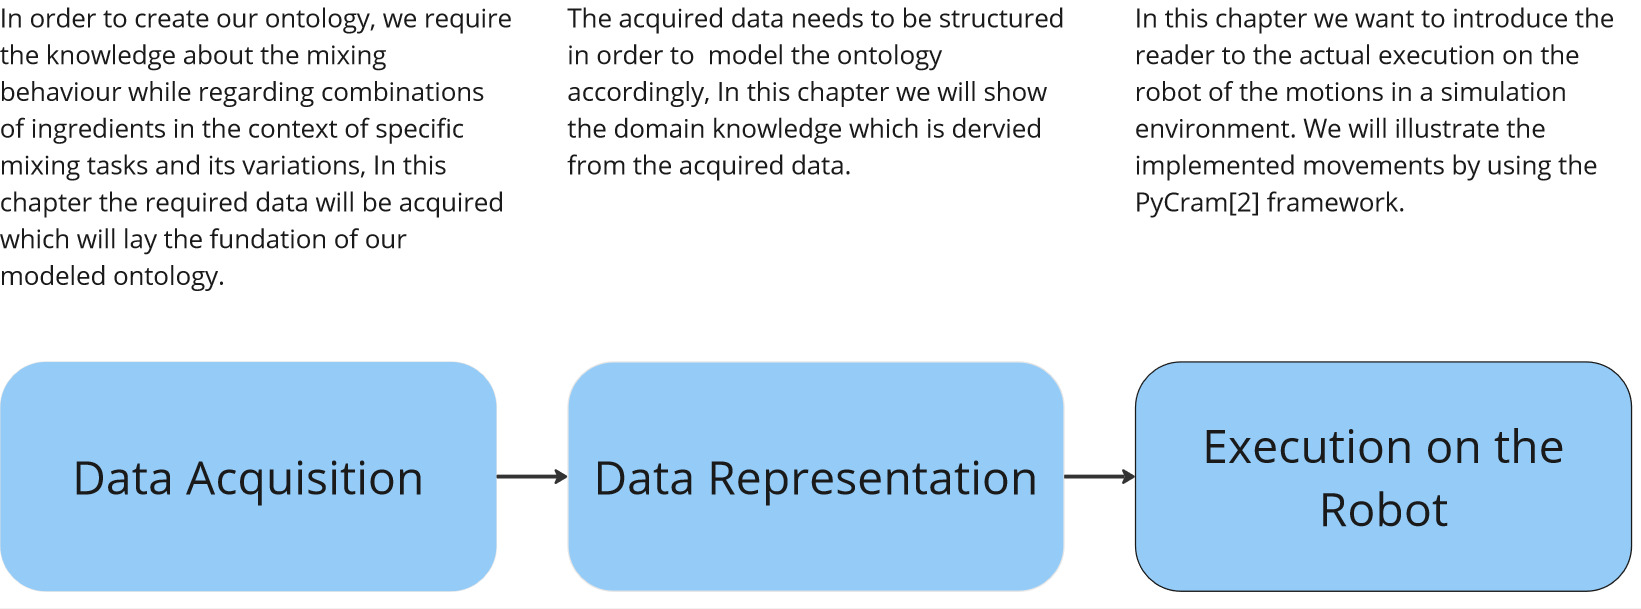
\includegraphics[scale=0.25]{Graphics/structure_overview.jpg}
    \caption{Structure overview}
\end{figure}